
\paragraph{Task paths}
We define the \textit{task-path} as a mapping of atomic tasks to ordered sequence of agents that work together to complete those tasks, $\formalTaskArc{}{}$. In completing an atomic task, the first agent in the sequence is the sink that received the associated composite task. The last agent is the detector that executes the atomic task. The sequence of agents in-between are those agents relaying the atomic task, their position in this sequence denoted by the subscript $i$ (See Figure \ref{fig:grid_concept}). So for a task path of depth $n$, we have;
\begin{equation}
	\functionTaskArc{}{} = \lbrace \functionSinkRoleAtomic{}{}, \functionRelayRole{i}{}{i+1}, \functionDetectorRole{}{} \rbrace_{i=2}^{n-1}
\end{equation}
\begin{figure}
	\centering 
	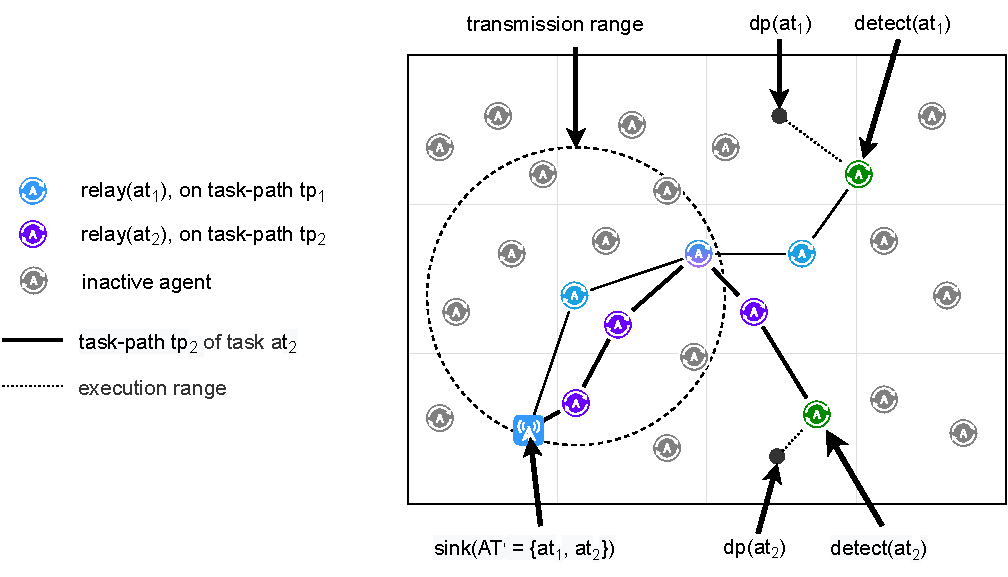
\includegraphics[width=0.75\linewidth, trim={25pt 0pt 24pt 0pt, clip}]{grid_concept}
	\caption[Task paths in a WSN]{\textbf{Task paths in a WSN} A sink $\varAgent{a}{} = \functionSinkRoleAtomic{}{}$ receives a composite task from an external agent, decomposes it into the single atomic task $\varAtomicTask{}{}$, and allocates this to the agent $\varAgent{b}{}$. $\varAgent{b}{}$ relays the task to $\varAgent{c}{}$, an agent in its current transmission range and its neighbourhood;  $\varAgent{b}{} = \functionRelayRole{2}{}{c}$. This agent then relays it to $\varAgent{d}{}$, and then finally to $\varAgent{e}{}$; $\varAgent{c}{} = \functionRelayRole{3}{}{d}$ and $\varAgent{d}{} = \functionRelayRole{4}{}{e}$. $\varAgent{e}{}$ then  completes the task; $\varAgent{e}{} = \functionDetectorRole{}{}$. The results of the tasks are then passed from $\varAgent{e}{}$ to  $\varAgent{d}{}$, $\varAgent{c}{}$, then $\varAgent{b}{}$ before arriving back at $\varAgent{a}{}$ for aggregation and return of the composite task results to the external agent that first made the request. This task path of $\varAtomicTask{}{}$ is then $\functionTaskArc{}{} = \lbrace \varAgent{a}{}, \varAgent{b}{}, \varAgent{c}{}, \varAgent{d}{}, \varAgent{e}{} \rbrace$.
	}
	\label{fig:grid_concept}
\end{figure}
